\documentclass[twocolumn]{aastex631}
\received{\today}
\shorttitle{APO Proposal}
\graphicspath{{figures/}}

\usepackage{lipsum}
\usepackage{physics}
\usepackage{multirow}
\usepackage{xspace}
\usepackage{natbib}
\usepackage{fontawesome5}
\usepackage{xcolor}
\usepackage{wrapfig}
\usepackage[figuresright]{rotating}

% remove indents in footnotes
\usepackage[hang,flushmargin]{footmisc} 

\newcommand{\todo}[1]{{\color{red}{[TODO: #1}]}}
\newcommand{\needcite}{{\color{magenta}{(needs citation)}}}
\newcommand{\placeholder}[1]{{\color{gray} \lipsum[#1]}}

% custom function for adding units
\makeatletter
\newcommand{\unit}[1]{%
    \,\mathrm{#1}\checknextarg}
\newcommand{\checknextarg}{\@ifnextchar\bgroup{\gobblenextarg}{}}
\newcommand{\gobblenextarg}[1]{\,\mathrm{#1}\@ifnextchar\bgroup{\gobblenextarg}{}}
\makeatother

\begin{document}

\title{{\Large Observing K2-138 to better constrain the planetary radius gap}\\\vspace{0.15cm}ASTR 581 APO Proposal}

% affiliations
\newcommand{\UW}{Department of Astronomy, University of Washington, Seattle, WA, 98195}

\author[0000-0001-6147-5761]{Tom Wagg}
\affiliation{\UW}

\correspondingauthor{Tom Wagg}
\email{tomwagg@uw.edu}

\section{Science Justification}
The observed planetary radius gap indicates a dearth of planets around $1.5-2.0 R_{\oplus}$ \citep{Fulton+2017,Fulton+2018}. Figure~\ref{fig:fulton_radius_gap} shows the figure from \citet{Fulton+2017} demonstrating the radius gap, which also indicates the typical uncertainty in the individual measurements. Previous work has suggested that this gap may be a result of photo-evaporation of planetary atmospheres \citep{Owen+2017} or other core-power mass-loss mechanisms \citep{Gupta+2019,Gupta+2020}. It is additionally possible that the magnetic fields of planets could affect the location of this radius gap \citep{Owen+2019} or even planetessimal impacts \citep{Wyatt+2020}. Therefore the exact location of this gap is crucial in better understanding planetary formation mechanisms.

The range of proposed theories and effects is indicative of the lack of precision in the measurement of the radius gap. The typical uncertainties on the planetary radii are such that the exact location of gap cannot currently be strongly stated \citep{Gandolfi+2019}. We propose to improve the measurement of this gap through the use of multi-transiting systems (systems with multiple transiting exoplanets). The advantage of this method is simple, each exoplanet is transiting the same star and this breaks several degeneracies present in single-transiting systems. The presence of multiple transiting planets allows one to better constrain the stellar radius, mass and other parameters and thus the planetary parameters, in particular the radii, as well.

\begin{figure}
    \centering
    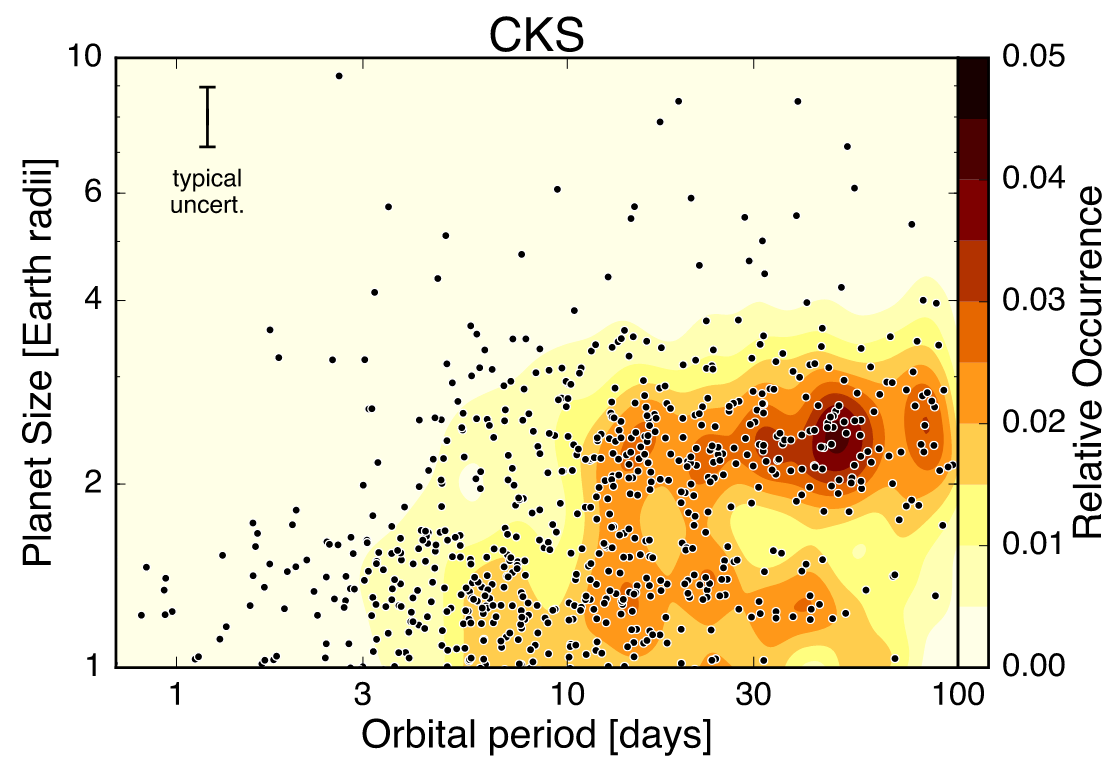
\includegraphics[width=\columnwidth]{fulton_2017_fig8.png}
    \caption{Figure 8 from \citep{Fulton+2017}, showing the observed radius gap. Note the typical uncertainty of the measurements.}
    \label{fig:fulton_radius_gap}
\end{figure}

We propose to use APO to observe the multi-transiting system K2-138 (see Table~\ref{tab:star}). First thought to contain 5 transiting exoplanets \citep{Christiansen+2018}, it is now confirmed to have a near-resonant chain of 6 transiting exoplanets \citep{Hardegree-Ullman+2021}. The many transiting planets with reasonably short orbital periods around a relatively bright makes this system ideal for better constraining the radius gap. K2-138 has been previously observed and characterised by other studies, which have focussed on general follow-up spectroscopy \citep{Lopez+2019} and investigating the composition of the planets \citep{Acuna+2022}. We seek to confirm and improve the transit timing of the innermost planets in the system, which will transit during our designated timeslot.

\begin{table}[htb]
    \centering
    \begin{tabular}{l|c} 
        \hline
        Property & Value \\
        \hline\hline
        Right Ascension & 23h15m47.77s \\
        Declination & $-10^\circ$ $50^\prime$ $59.06^{\prime\prime}$ \\
        V-band Magnitude & 12.25 \\
        Stellar Type & K1V \\
        Distance & 202 pc \\
        \hline
    \end{tabular}
    \caption{Properties of the proposed target star KS-138}
    \label{tab:star}
\end{table}

Observations from APO will help to characterise the lightcurve of K2-138, in particular the transit timing for planets KS-138b and KS-138c, and therefore directly contribute to improving our measurement of the planetary radius gap.

\section{Proposed Observations}

\paragraph{Timing} We propose to observe two transits of K2-138 on 2022-09-18 and 2022-09-19 by K2-138c and K2-138b respectively using ARCTIC in order to better characterise the lightcurve. In particular, we aim to focus on the ingress and egress of the transit. The transit durations are 1.95 and 2.34 hours respectively and we need to observe the flux for 30 minutes prior to and after the transit. We therefore request two half-nights that include the transits (see Table~\ref{tab:transits}).

\begin{figure}[htb]
    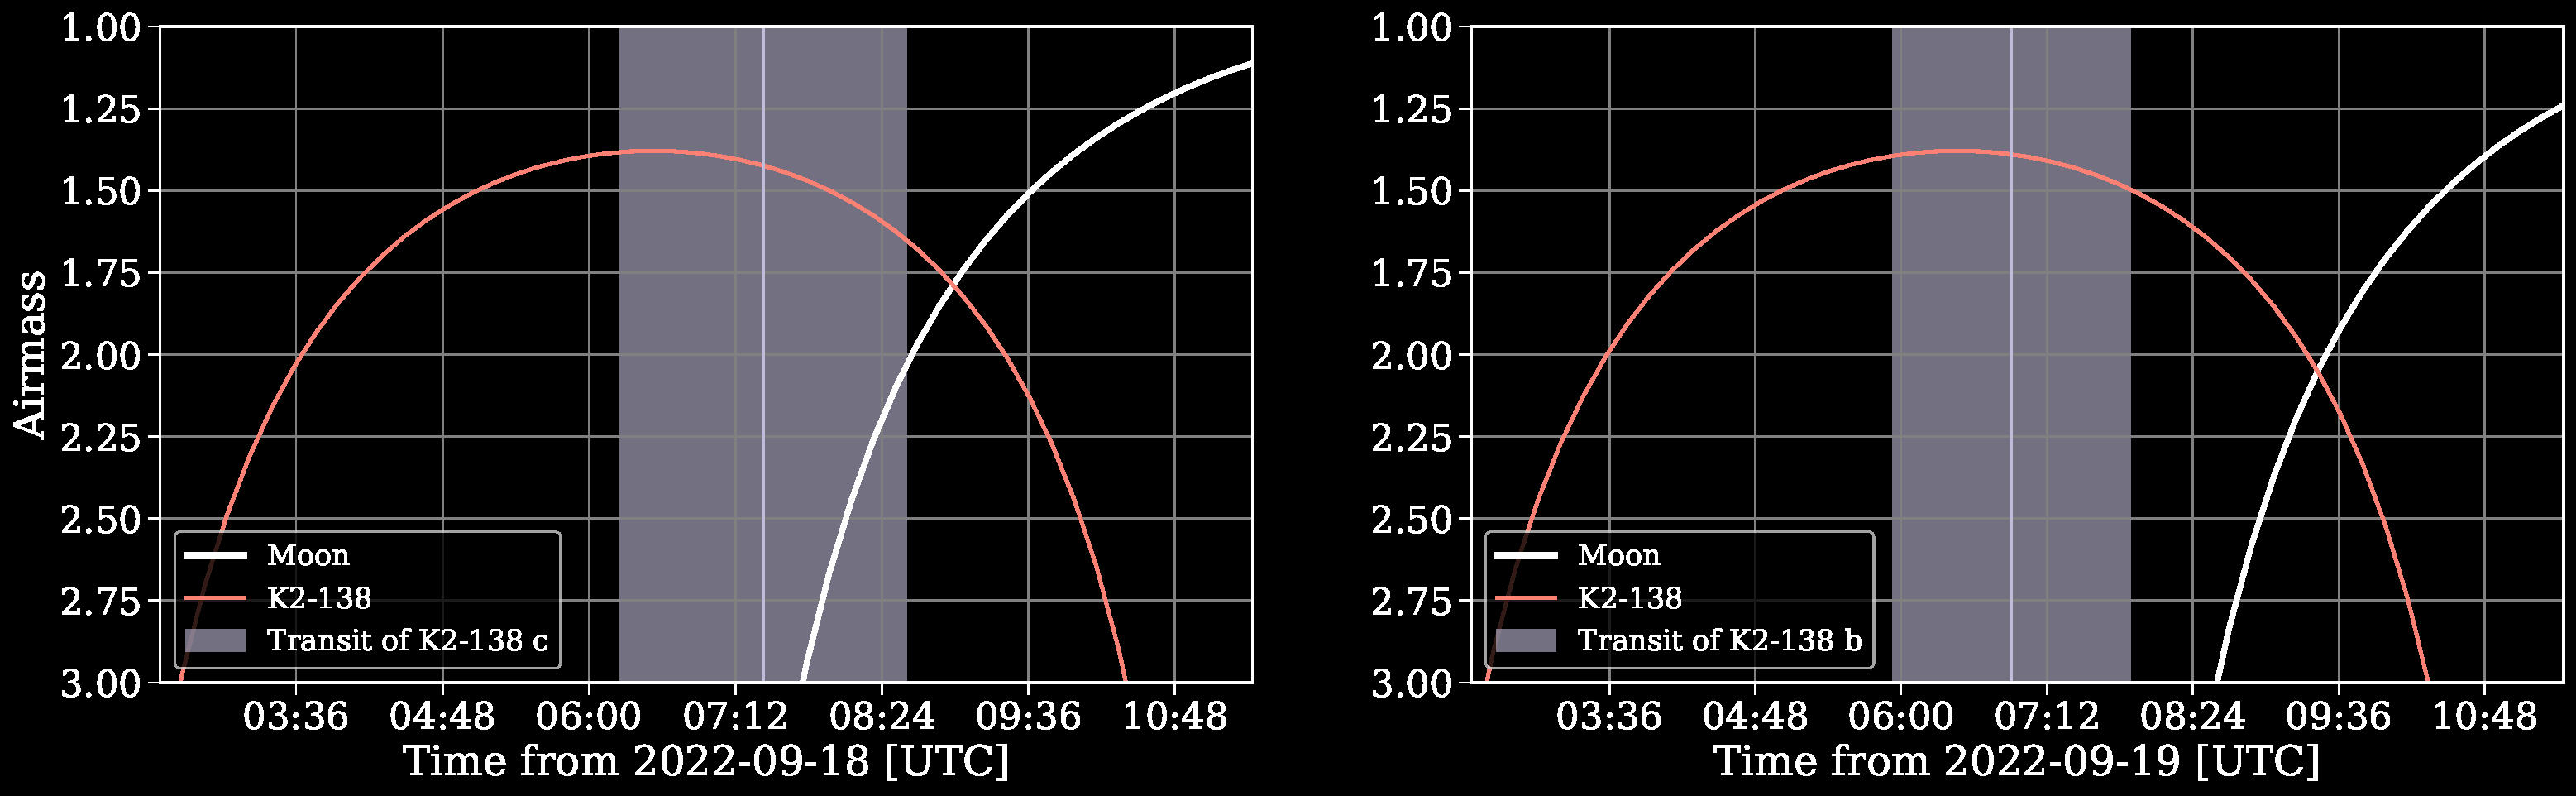
\includegraphics[width=\columnwidth]{observable_transits.pdf}
    \caption{Proposed transit observation for K2-138. Airmass over time for two separate observing nights. Grey shaded regions indicate sunset and twilight times. Orange shaded region indicates transit period and orange line represents the time of mid-transit.}
\end{figure}

\begin{table}[htb]
    \centering
    \begin{tabular}{l|c|c|c|c} 
        \hline
        Planet & Transit Date & Ingress & Mid-Transit & Egress \\
        \hline\hline
        KS-138c & 2022-09-18 & 05:56 & 06:54 & 07:53 \\
        KS-138b & 2022-09-19 & 06:27 & 07:26 & 08:24 \\
        \hline
    \end{tabular}
    \caption{Transit information for planets around KS-138 in UTC}
    \label{tab:transits}
\end{table}

\paragraph{Observing plan} We intend to use to narrow-band ARCTIC H-$\alpha$ filter\footnote{\url{http://filters.apo.nmsu.edu/index.php}} for our observations of these transits. We will use this filter in order to prevent saturation that can occur when using broadband filters with a star of this magnitude\footnote{\url{https://www.apo.nmsu.edu/arc35m/Instruments/ARCTIC/\#3p6}}. We will observe with a cadence of 2 minutes and an exposure time of 3-5 seconds, using the default medium readout time of 25 seconds\footnote{\url{https://www.apo.nmsu.edu/arc35m/Instruments/ARCTIC/\#3p1}}. Since one of the main purposes of these observations is to better characterise the lightcurve and the exact timing of the transits, we will increase the cadence to 30 seconds for 20 minutes around the ingress and egress of the transits, using the fast readout time of 11 seconds (see Table~\ref{tab:settings}).

\begin{table}[htb]
    \centering
    \begin{tabular}{l|c|c} 
        \hline
        \multicolumn{1}{l|}{\multirow{2}{*}{Setting}} & \multicolumn{2}{c}{Value}                                         \\ \cline{2-3} 
\multicolumn{1}{l|}{}                         & \multicolumn{1}{c|}{Regular} & \multicolumn{1}{c}{Ingress/Egress} \\
        \hline\hline
        Exposure Time & 3-5 seconds & 3-5 seconds\\
        Filter & H-$\alpha$ & H-$\alpha$ \\
        Readout time & 25 seconds & 11 seconds \\
        Cadence & 2 minutes & 30 seconds \\
        \hline
    \end{tabular}
    \caption{ARCTIC Settings for observations. We increase use the ARCTIC fast readout time and increase the cadence for 20 minutes around transit ingress and egress in order to better characterise transit timing variations.}
    \label{tab:settings}
\end{table}

\paragraph{Calibrations} Since we are using a narrowband (H-$\alpha$) filter for these observations, we will use the bright quartz lamp to take flats prior to our observations\footnote{\url{https://www.apo.nmsu.edu/arc35m/Instruments/ARCTIC/\#4p2}}. We shall take several flats, median combine the results and then apply them to our final image to account for different quantum efficiency in the CCD pixels. We will not apply dark subtraction to our images since ARCTIC guidelines suggest against this for exposure times shorter than 30 seconds\footnote{\url{https://www.apo.nmsu.edu/arc35m/Instruments/ARCTIC/\#4p3}}. We will still however use bias frames to account for fixed-pattern noise in the detector.

\begin{figure*}
    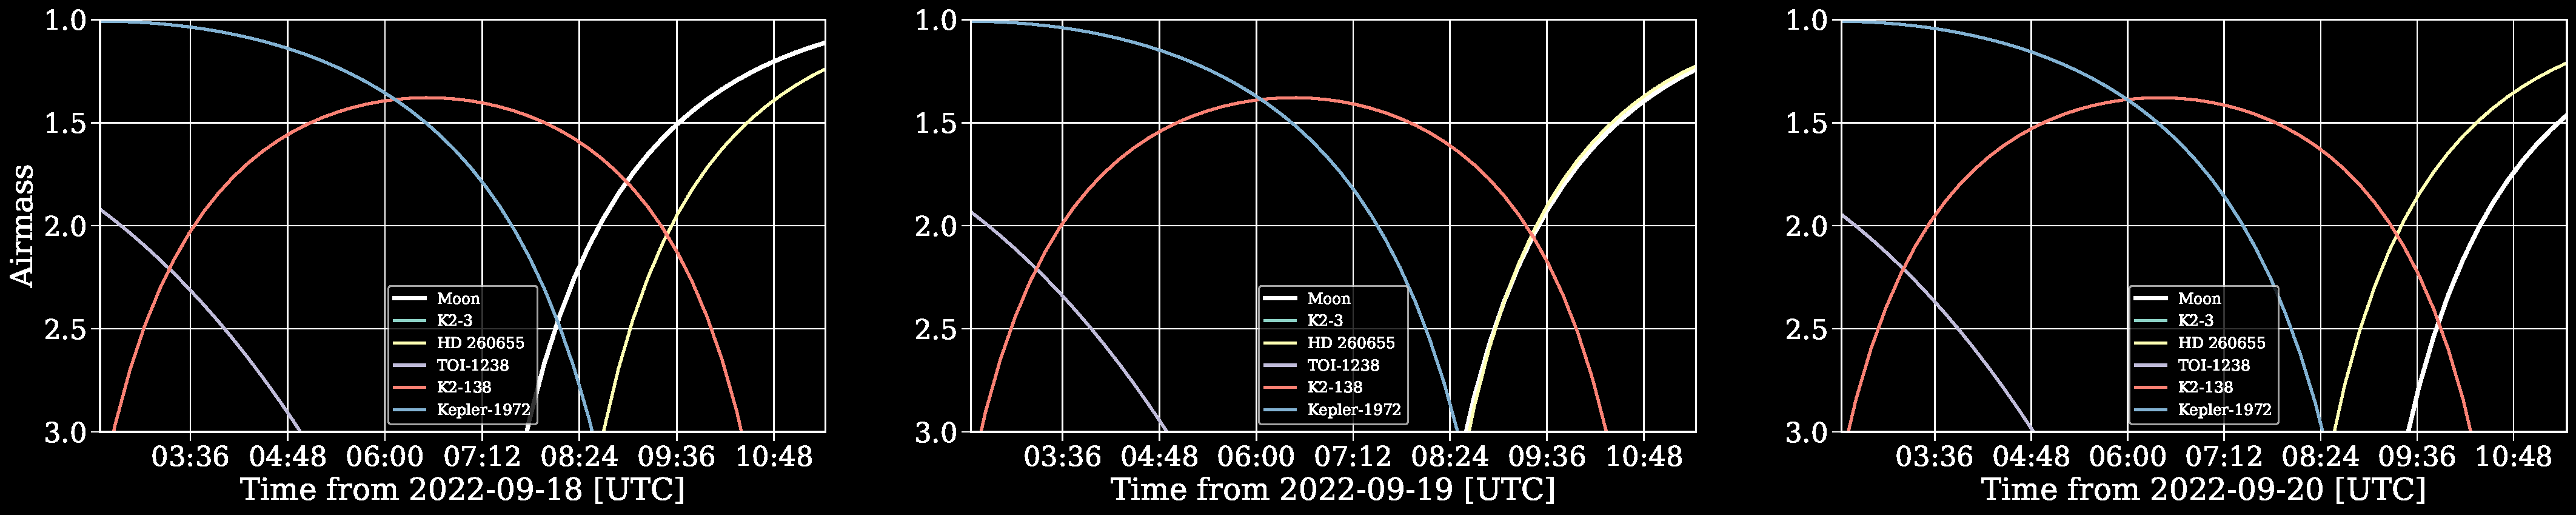
\includegraphics[width=\textwidth]{potential_systems.pdf}
    \caption{Airmass over time for different potentially observable multi-transiting systems. Different panels correspond to different observing nights. Shaded grey regions indicate twilight times and sunset.}
    \label{fig:potential_systems}
\end{figure*}

\section{Alternative Observations}

[\textit{Note: I don't think this section belongs in a \emph{real} proposal but I investigated other things I wanted to share what I'd done haha}]

We considered several multi-transiting systems for this proposal, taking into account the constraints of both whether the system is observable during the allotted time period and whether it is transitting. As we show in Figure~\ref{fig:potential_systems}, of the five systems that we considered, only Kepler-1972 \citep{Leleu+2022} and K2-138 were observable for a significant fraction of time. Unfortunately none of the planets in the Kepler-1972 transit during the given time period and hence we selected K2-138 as our target.

We did additionally consider whether we could use ARCES to perform high-resolution spectroscopy of either system whilst out of transit in case the transit time periods were unavailable. However, both systems have expected radial velocities of the order of $\sim 1 \unit{km}{s^{-1}}$. We find that this would be too low for ARCES to resolve since its resolution is $R = 31500$ and this implies that the minimum resolvable radial velocity would be
\begin{equation}
    \Delta v_{\rm min} = \frac{c}{R} \approx \frac{3 \times 10^{5} \unit{km}{s^{-1}}}{31500} \approx 10 \unit{km}{s^{-1}}.
\end{equation}
It may be possible that we could use ARCES to investigate particular spectral lines that would indicate the stars' metallicities, surface gravities or stellar activity levels. However, we lack the experience for reducing these spectra and hence focus on imaging instead.

\bibliographystyle{aasjournal}
\bibliography{proposal}{}

\end{document}